\chapter{Mecânica lagrangiana}\label{ch:b3:lagrangian-mechanics}

Tente escrever a lei de Newton para um pêndulo duplo: duas forças de
tração, nenhuma delas conhecida de antemão, ambas mudando de direção a
cada instante, e quatro equações escalares a desembaraçar só para
descobrir como evoluem dois ângulos. Faça agora o mesmo para uma conta
num aro que gira, para uma cadeia de molas acopladas, para um braço
robótico. As forças que mantêm um sistema coeso --- hastes, trilhos,
dobradiças --- não realizam trabalho algum e, ainda assim, o método de
Newton nos obriga a carregá-las por todo o cálculo. Este capítulo
apresenta a reformulação que Lagrange publicou em 1788: descrever o
sistema pelas poucas coordenadas que de fato podem variar, escrever uma
única função $L = E_k - E_p$ e deixar que uma só receita produza as
equações de movimento em quaisquer coordenadas, com todas as hastes e
trilhos já eliminados. Melhor ainda, a nova formulação torna visível o
que a de Newton esconde: cada simetria de $L$ fornece uma grandeza
conservada --- o momento, da uniformidade do espaço; a energia, da
uniformidade do tempo --- resultado de Emmy Noether que se tornou o
princípio organizador da física muito além da mecânica.

\section{Das forças às coordenadas}

\begin{definition}[Vínculos, graus de liberdade, coordenadas generalizadas]\label{def:b3:lagrangian-mechanics:coordinates}
\index{vínculo}\index{graus de liberdade}\index{coordenadas generalizadas}
Um \emph{vínculo} é uma condição geométrica imposta às posições de um
sistema --- uma conta permanece em seu arame, a haste de um pêndulo
mantém comprimento fixo, duas rodas de um mesmo eixo giram juntas. Um
vínculo que se exprime como uma equação
$f(\vect r_1, \dots, \vect r_N, t) = 0$ entre as coordenadas (e
eventualmente o tempo) diz-se \emph{holônomo}. O número de maneiras
independentes pelas quais a configuração ainda pode variar é o número
de \emph{graus de liberdade} $n$; qualquer conjunto de $n$ grandezas
independentes $q_1, \dots, q_n$ que fixe a configuração por completo é
um conjunto de \emph{coordenadas generalizadas} --- ângulos,
comprimentos ou qualquer mistura conveniente. Suas derivadas temporais
$\dot q_1, \dots, \dot q_n$ são as
\emph{velocidades generalizadas}\index{velocidades generalizadas}.
\end{definition}

\begin{example}[Contagem dos graus de liberdade]\label{ex:b3:lagrangian-mechanics:counting}
Um ponto sobre uma mesa: $n = 2$. Um pêndulo plano de comprimento
fixo: um ângulo, $n = 1$. Um pêndulo duplo: dois ângulos,
$n = 1 + 1 = 2$. Uma conta num aro rígido: um ângulo, $n = 1$ ---
mesmo que o próprio aro seja forçado a girar, pois a rotação imposta
não acrescenta liberdade alguma. Um corpo rígido livre no espaço: três
coordenadas de seu centro mais três ângulos, $n = 6$. Um gás de $N$
moléculas livres (pontuais): $n = 3N$. Cada \omterm{def:b3:lagrangian-mechanics:coordinates}{vínculo} holônomo suprime um
grau de liberdade: dois pontos unidos por uma haste têm
$3 + 3 - 1 = 5$.
\end{example}

\begin{omfigure}
\begin{tikzpicture}[font=\small, >=Stealth]
  % (a) plane pendulum
  \begin{scope}
    \draw[thick] (-1,0) -- (1,0);
    \foreach \i in {-0.8,-0.5,-0.2,0.1,0.4,0.7} \draw (\i,0) -- (\i+0.18,0.16);
    \fill (0,0) circle (1.5pt);
    \draw[dashed] (0,0) -- (0,-2.2);
    \draw[thick] (0,0) -- (-55:2.1);
    \fill[omDef] (-55:2.1) circle (3pt);
    \draw[->] (0,-1.0) arc (-90:-55:1.0);
    \node at (-72:1.35) {$\theta$};
    \node at (-55:2.5) {$m$};
    \node at ($(-55:1.35)+(0.28,0.12)$) {$\ell$};
    \node at (0,-2.9) {uma coordenada: $\theta$};
  \end{scope}
  % (b) bead on rotating hoop
  \begin{scope}[xshift=6.2cm]
    \coordinate (C) at (0,-2.35);
    \draw[thick] (C) circle (1.55);
    \draw[dashed] (0,-0.3) -- (0,-4.6);
    \draw[->, thick] (0.35,-0.15) arc (20:160:0.37);
    \node at (0,0.25) {$\omega$};
    \fill (C) circle (1pt);
    \draw (C) -- ++(-50:1.55);
    \fill[omDef] ($(C)+(-50:1.55)$) circle (3pt);
    \draw[->] ($(C)+(0,-0.85)$) arc (-90:-50:0.85);
    \node at ($(C)+(-70:1.18)$) {$\theta$};
    \node at ($(C)+(-38:2.0)$) {$m$};
    \draw (C) -- ++(135:1.55);
    \node at (-1.35,-1.35) {$R$};
    \node at (0,-4.95) {uma coordenada: $\theta$};
  \end{scope}
  % (c) double pendulum
  \begin{scope}[xshift=11.4cm]
    \draw[thick] (-0.9,0) -- (0.9,0);
    \foreach \i in {-0.7,-0.4,-0.1,0.2,0.5} \draw (\i,0) -- (\i+0.18,0.16);
    \fill (0,0) circle (1.5pt);
    \draw[dashed] (0,0) -- (0,-1.7);
    \draw[thick] (0,0) -- (-65:1.5) coordinate (m1);
    \fill[omDef] (m1) circle (2.6pt);
    \draw[dashed] (m1) -- ++(0,-1.5);
    \draw[thick] (m1) -- ++(-40:1.5) coordinate (m2);
    \fill[omThm] (m2) circle (2.6pt);
    \draw[->] (0,-0.8) arc (-90:-65:0.8);
    \node at (-80:1.1) {$\theta_1$};
    \draw[->] ($(m1)+(0,-0.75)$) arc (-90:-40:0.75);
    \node at ($(m1)+(-68:1.05)$) {$\theta_2$};
    \node at (0.3,-3.4) {duas coordenadas: $\theta_1, \theta_2$};
  \end{scope}
\end{tikzpicture}

{\small \omterm{def:b3:lagrangian-mechanics:coordinates}{Coordenadas generalizadas}: cada sistema é descrito pelos
ângulos que de fato podem variar, e não pelas coordenadas cartesianas
de suas massas. As trações das hastes e a força normal do aro nunca
aparecem.}
\end{omfigure}

\section{O princípio da mínima ação}

\begin{definition}[Lagrangiana e ação]\label{def:b3:lagrangian-mechanics:action}
\index{lagrangiana}\index{ação}
A \emph{lagrangiana} de um sistema mecânico cujas forças derivam de uma
energia potencial $E_p$ é a função das coordenadas, das velocidades e,
eventualmente, do tempo
\[
L(q, \dot q, t) = E_k - E_p ,
\]
energia cinética \emph{menos} energia potencial, ambas expressas nas
\omterm{def:b3:lagrangian-mechanics:coordinates}{coordenadas generalizadas}. A \emph{ação} de um movimento concebível
$q(t)$ entre extremidades fixas $q(t_1)$ e $q(t_2)$ é o número
\[
S[q] = \int_{t_1}^{t_2} L\big(q(t), \dot q(t), t\big)\,\dd t .
\]
$S$ é um \emph{funcional}: devora um caminho inteiro e devolve um único
número, em joule-segundos --- a unidade da constante de Planck.
\end{definition}

\begin{theorem}[Princípio de Hamilton e equações de Euler--Lagrange]\label{thm:b3:lagrangian-mechanics:euler-lagrange}
\index{princípio de Hamilton}\index{equações de Euler--Lagrange}\index{mínima ação}
Entre todos os movimentos concebíveis que unem as mesmas duas
extremidades no mesmo tempo, o movimento real é aquele que torna a \omterm{def:b3:lagrangian-mechanics:action}{ação}
\emph{estacionária} (\emph{princípio de Hamilton}, ou princípio da
\emph{\omterm{thm:b3:lagrangian-mechanics:euler-lagrange}{mínima ação}}). De modo equivalente, o movimento obedece às
\emph{\omterm{thm:b3:lagrangian-mechanics:euler-lagrange}{equações de Euler--Lagrange}}
\[
\frac{\dd}{\dd t}\frac{\partial L}{\partial\dot q_i}
 - \frac{\partial L}{\partial q_i} = 0 ,
\qquad i = 1, \dots, n :
\]
uma equação de segunda ordem por grau de liberdade, quaisquer que
sejam as coordenadas escolhidas.
\end{theorem}

\begin{proof}
Deforme o caminho: $q_i(t) \to q_i(t) + \delta q_i(t)$ com
$\delta q_i(t_1) = \delta q_i(t_2) = 0$. Em primeira ordem,
\[
\delta S = \int_{t_1}^{t_2}\sum_i\Big(
  \frac{\partial L}{\partial q_i}\,\delta q_i
 + \frac{\partial L}{\partial\dot q_i}\,\delta\dot q_i\Big)\dd t
 = \int_{t_1}^{t_2}\sum_i\Big(
  \frac{\partial L}{\partial q_i}
 - \frac{\dd}{\dd t}\frac{\partial L}{\partial\dot q_i}\Big)\delta q_i\,\dd t ,
\]
após integrar o segundo termo por partes ($\delta\dot q_i =
\dd(\delta q_i)/\dd t$) e descartar o termo de fronteira, que se anula
nas extremidades fixas. Se $\delta S = 0$ para \emph{toda} deformação,
o colchete deve anular-se a cada instante e para cada $i$ --- fosse ele
positivo em algum ponto, uma saliência $\delta q_i$ concentrada ali
daria $\delta S \neq 0$. A recíproca lê-se na mesma linha.
\end{proof}

\begin{omfigure}
\begin{tikzpicture}[font=\small, >=Stealth]
  \draw[->] (0,0) -- (7.6,0) node[right] {$t$};
  \draw[->] (0,0) -- (0,3.4) node[above] {$q$};
  \fill (0.8,0.7) circle (2pt) node[below left] {$q(t_1)$};
  \fill (6.8,2.3) circle (2pt) node[above right] {$q(t_2)$};
  \draw[omDef, very thick] (0.8,0.7) .. controls (2.6,2.6) and (5.0,1.4) .. (6.8,2.3);
  \draw[omExo, dashed] (0.8,0.7) .. controls (2.2,0.6) and (5.4,0.9) .. (6.8,2.3);
  \draw[omExo, dashed] (0.8,0.7) .. controls (3.0,3.6) and (5.2,2.9) .. (6.8,2.3);
  \node[omDef] at (1.9,3.35) {caminho real};
  \draw[->, omDef] (2.25,3.15) -- (2.85,2.3);
  \node[omExo] at (3.4,0.42) {caminhos variados};
  \draw[<->] (4.1,1.62) -- (4.1,2.62);
  \node at (4.55,2.15) {$\delta q$};
\end{tikzpicture}

{\small O princípio de Hamilton: entre todos os caminhos com as mesmas
extremidades e a mesma duração, o real torna $S = \int L\,\dd t$
estacionária --- deformações $\delta q$ de primeira ordem alteram $S$
apenas em segunda ordem.}
\end{omfigure}

\begin{proposition}[Newton recuperado]\label{prop:b3:lagrangian-mechanics:newton}
Para uma partícula em coordenadas cartesianas, $L = \tfrac12 m(\dot x^2 +
\dot y^2 + \dot z^2) - E_p(x,y,z)$, e as \omterm{thm:b3:lagrangian-mechanics:euler-lagrange}{equações de Euler--Lagrange}
dão $m\ddot x = -\partial E_p/\partial x$ e o análogo para $y$ e $z$:
exatamente $m\vect a = \vect F$. As mecânicas \omterm{def:b3:lagrangian-mechanics:action}{lagrangiana} e newtoniana
concordam sempre que ambas se aplicam; a nova forma simplesmente
sobrevive a uma mudança de coordenadas, o que as equações em
componentes de Newton não fazem.
\end{proposition}

\begin{proof}
$\partial L/\partial\dot x = m\dot x$, $\partial L/\partial x =
-\partial E_p/\partial x$; a equação de Euler--Lagrange é
$\dd(m\dot x)/\dd t + \partial E_p/\partial x = 0$.
\end{proof}

\begin{remark}[Por que as forças de vínculo desaparecem]\label{rem:b3:lagrangian-mechanics:constraints}
A tração de uma haste, a força normal de um trilho, agem
perpendicularmente a todo deslocamento que o \omterm{def:b3:lagrangian-mechanics:coordinates}{vínculo} permite: elas não
realizam trabalho em nenhum movimento compatível com o \omterm{def:b3:lagrangian-mechanics:coordinates}{vínculo}. Como a
\omterm{def:b3:lagrangian-mechanics:action}{ação} é construída a partir de energias avaliadas apenas sobre tais
movimentos, essas forças jamais entram em $L$ --- eis o milagre prático
do método. A justificativa geral (o princípio dos trabalhos virtuais de
d'Alembert) é aqui admitida; para todos os sistemas deste livro, a
receita abaixo pode ser conferida diretamente contra Newton, como a
\cref{prop:b3:lagrangian-mechanics:newton} começou a fazer. Se a
própria força de \omterm{def:b3:lagrangian-mechanics:coordinates}{vínculo} for desejada --- a haste vai romper? ---
volta-se a Newton apenas para essa força, com o movimento já conhecido.
\end{remark}

\begin{method}[A receita lagrangiana]\label{met:b3:lagrangian-mechanics:recipe}
(1) Conte os \omterm{def:b3:lagrangian-mechanics:coordinates}{graus de liberdade} e escolha coordenadas $q_i$ --- ângulos
para rotações, abscissas ao longo de trilhos. (2) Exprima as posições
$\vect r(q_i, t)$, derive para obter as velocidades e escreva $E_k$;
escreva $E_p$. (3) $L = E_k - E_p$, descartando qualquer constante
aditiva. (4) Uma equação de Euler--Lagrange por coordenada. (5) Antes
de resolver, colha as grandezas conservadas: as \omterm{def:b3:lagrangian-mechanics:momentum}{coordenadas cíclicas}
(\cref{def:b3:lagrangian-mechanics:momentum}) e a \omterm{prop:b3:lagrangian-mechanics:energy}{função energia}
(\cref{prop:b3:lagrangian-mechanics:energy}). (6) Verifique os limites:
pequenos ângulos, rotação desligada, casos particulares conhecidos.
\end{method}

\begin{example}[O pêndulo, em três linhas]\label{ex:b3:lagrangian-mechanics:pendulum}
Uma coordenada $\theta$; $\vect v = \ell\dot\theta\,\vect e_\theta$,
logo $E_k = \tfrac12 m\ell^2\dot\theta^2$ e
$E_p = -mg\ell\cos\theta$. Então
$L = \tfrac12 m\ell^2\dot\theta^2 + mg\ell\cos\theta$ e
$\dd(m\ell^2\dot\theta)/\dd t = -mg\ell\sin\theta$:
\[
\ddot\theta = -\frac{g}{\ell}\sin\theta ,
\]
a equação que o volume do primeiro ano obteve a partir do torque do
peso --- sem que a tração fosse mencionada uma única vez.
\end{example}

\begin{example}[Conta num aro que gira]\label{ex:b3:lagrangian-mechanics:hoop}
Uma conta de massa $m$ desliza sobre um aro circular vertical de raio
$R$ forçado a girar em torno de seu diâmetro vertical com $\omega$
constante (\cref{ex:b3:lagrangian-mechanics:counting}). Uma coordenada,
o ângulo polar $\theta$ medido a partir do ponto mais baixo. A
velocidade da conta tem uma componente $R\dot\theta$ ao longo do aro e
outra $\omega R\sin\theta$ devida à rotação imposta, perpendicular a
ele:
\[
L = \tfrac12 mR^2\dot\theta^2 + \tfrac12 m\omega^2R^2\sin^2\theta
 + mgR\cos\theta ,
\qquad
mR^2\ddot\theta = m\omega^2R^2\sin\theta\cos\theta - mgR\sin\theta .
\]
Equilíbrios em que $\ddot\theta = 0$: o ponto mais baixo $\theta = 0$
(e o mais alto, sempre instável) e, quando $\omega^2 > g/R$, um novo
par $\cos\theta_{\text{eq}} = g/\omega^2R$. Escrevendo a equação como
$mR^2\ddot\theta = -\dd U_{\text{eff}}/\dd\theta$ com a
\emph{energia potencial efetiva}\index{energia potencial efetiva}
\[
U_{\text{eff}}(\theta) = -mgR\cos\theta
 - \tfrac12 m\omega^2R^2\sin^2\theta
\]
torna a geometria visível: abaixo da taxa crítica
$\omega_{\text{c}} = \sqrt{g/R}$ o fundo é um poço; acima dela, o fundo
se torna um cume e a conta se acomoda na encosta, subindo mais quanto
mais rápido o aro gira --- o princípio do regulador centrífugo que
governava as máquinas a vapor.
\end{example}

\begin{omfigure}
\begin{tikzpicture}
  \begin{axis}[omaxis, axis x line=bottom, axis y line=left,
    width=11.4cm, height=5.6cm, xmin=-180, xmax=180,
    ymin=-1.65, ymax=1.2, xlabel={$\theta$ (graus)},
    xlabel style={at={(axis description cs:0.5,-0.1)}, anchor=north},
    ylabel={$U_{\text{eff}}/mgR$}, xtick={-180,-90,0,90,180}, ytick=\empty,
    clip=false,
    legend style={font=\scriptsize, at={(0.5,-0.32)}, anchor=north,
      draw=none, fill=none, legend columns=2}]
    \addplot[omDef, thick, domain=-180:180, samples=90]
      {-cos(x) - 0.25*sin(x)^2};
    \addlegendentry{$\omega^2 = g/2R$ (lento): poço em $\theta = 0$}
    \addplot[omThm, thick, domain=-180:180, samples=90]
      {-cos(x) - 1.0*sin(x)^2};
    \addlegendentry{$\omega^2 = 2g/R$ (rápido): poços em $\pm 60^\circ$}
    \fill[omThm] (axis cs:60,-1.25) circle (1.8pt);
    \fill[omThm] (axis cs:-60,-1.25) circle (1.8pt);
    \fill[omDef] (axis cs:0,-1) circle (1.8pt);
  \end{axis}
\end{tikzpicture}

{\small A \omterm{ex:b3:lagrangian-mechanics:hoop}{energia potencial efetiva} da conta no aro que gira. Quando
$\omega$ ultrapassa $\sqrt{g/R}$, o poço único do fundo se desdobra em
dois poços simétricos: o ângulo de equilíbrio cresce com a rotação.}
\end{omfigure}

\section{Simetrias e leis de conservação}

\begin{definition}[Momento generalizado, coordenada cíclica]\label{def:b3:lagrangian-mechanics:momentum}
\index{momento generalizado}\index{coordenada cíclica}
O \emph{momento generalizado} conjugado à coordenada $q_i$ é
\[
p_i = \frac{\partial L}{\partial\dot q_i} .
\]
Para uma coordenada cartesiana, é o momento linear ordinário $m\dot x$;
para um ângulo, é um momento angular. Uma coordenada que não aparece em
$L$ (embora sua velocidade apareça) diz-se \emph{cíclica}.
\end{definition}

\begin{proposition}[Coordenadas cíclicas dão leis de conservação]\label{prop:b3:lagrangian-mechanics:cyclic}
Se $q_i$ é cíclica, seu momento conjugado se conserva:
$\partial L/\partial q_i = 0$ implica $\dd p_i/\dd t = 0$. Escolher as
coordenadas de modo que o maior número possível delas seja cíclica é o
passo isolado mais eficaz na resolução de um problema de mecânica.
\end{proposition}

\begin{proof}
Imediato, a partir da equação de Euler--Lagrange para $q_i$.
\end{proof}

\begin{example}[Força central, resolvida por inspeção]\label{ex:b3:lagrangian-mechanics:central}
Uma partícula num potencial central $E_p(r)$, em coordenadas polares no
seu plano de movimento:
\[
L = \tfrac12 m(\dot r^2 + r^2\dot\varphi^2) - E_p(r) .
\]
$\varphi$ é cíclica, de modo que $p_\varphi = mr^2\dot\varphi$ --- o
momento angular --- se conserva: a lei das áreas de Kepler, que o
volume do primeiro ano deduziu da equação do torque, cai aqui antes de
qualquer equação ser resolvida. A equação radial restante é
$m\ddot r = mr\dot\varphi^2 - E_p'(r)$, isto é, o movimento
unidimensional na \omterm{ex:b3:lagrangian-mechanics:hoop}{energia potencial efetiva}
$E_p(r) + p_\varphi^2/2mr^2$ daquele volume.
\end{example}

\begin{theorem}[Teorema de Noether]\label{thm:b3:lagrangian-mechanics:noether}
\index{teorema de Noether}\index{simetria}
A toda simetria contínua da \omterm{def:b3:lagrangian-mechanics:action}{lagrangiana} corresponde uma grandeza
conservada. Precisamente: se o deslocamento
$q_i \to q_i + \varepsilon\,K_i(q)$ deixa $L$ inalterada em primeira
ordem em $\varepsilon$ para todos os movimentos, então
\[
Q = \sum_i p_i\,K_i(q)
\]
é constante ao longo de todo movimento real. A uniformidade do espaço
(invariância por translação) fornece o momento linear; a isotropia do
espaço (invariância por rotação) fornece o momento angular; a
uniformidade do tempo fornece a energia
(\cref{prop:b3:lagrangian-mechanics:energy}).
\end{theorem}

\begin{proof}
A invariância em primeira ordem significa
$0 = \delta L = \sum_i\big(\partial_{q_i}L\,K_i +
\partial_{\dot q_i}L\,\dot K_i\big)\varepsilon$. Sobre um movimento
real, $\partial_{q_i}L = \dot p_i$ por Euler--Lagrange, de modo que o
colchete vale $\sum_i(\dot p_iK_i + p_i\dot K_i) = \dd Q/\dd t$. Uma
\omterm{def:b3:lagrangian-mechanics:momentum}{coordenada cíclica} é o caso particular $K_i = \delta_{ij}$. O caso do
deslocamento temporal exige o cálculo separado da
\cref{prop:b3:lagrangian-mechanics:energy}; o teorema completo, para
transformações que também alteram $t$ ou modificam $L$ por uma derivada
total, é demonstrado nos cursos de mecânica analítica e aqui admitido
nessa generalidade.
\end{proof}

\begin{proposition}[A função energia]\label{prop:b3:lagrangian-mechanics:energy}
\index{função energia}
Ao longo de qualquer movimento, a \emph{\omterm{prop:b3:lagrangian-mechanics:energy}{função energia}}
\[
h = \sum_i \dot q_i\,\frac{\partial L}{\partial\dot q_i} - L
\qquad\text{obedece a}\qquad
\frac{\dd h}{\dd t} = -\frac{\partial L}{\partial t} .
\]
Se $L$ não depende explicitamente do tempo, $h$ se conserva. Se, além
disso, as relações $\vect r(q)$ entre posições e coordenadas não
envolvem o tempo --- nenhuma rotação imposta, nenhum apoio móvel ---
então $E_k$ é uma forma quadrática nas $\dot q_i$ e $h = E_k + E_p$: a
energia mecânica. Com um \omterm{def:b3:lagrangian-mechanics:coordinates}{vínculo} dependente do tempo, $h$ ainda se
conserva quando $\partial L/\partial t = 0$, mas \emph{não} é a
energia: o motor que impõe o \omterm{def:b3:lagrangian-mechanics:coordinates}{vínculo} troca trabalho com o sistema.
\end{proposition}

\begin{proof}
$\dd h/\dd t = \sum_i(\ddot q_ip_i + \dot q_i\dot p_i) -
\sum_i(\partial_{q_i}L\,\dot q_i + \partial_{\dot q_i}L\,\ddot q_i) -
\partial_tL$. Os termos em $\ddot q_i$ se cancelam; as \omterm{thm:b3:lagrangian-mechanics:euler-lagrange}{equações de
Euler--Lagrange} transformam $\dot p_i$ em $\partial_{q_i}L$, cancelando
o par seguinte; resta $-\partial_tL$. Se $E_k = \tfrac12\sum a_{jk}(q)\dot
q_j\dot q_k$, a identidade de Euler para formas quadráticas dá $\sum\dot
q_i\,\partial E_k/\partial\dot q_i = 2E_k$, logo $h = 2E_k - (E_k - E_p)
= E_k + E_p$.
\end{proof}

\begin{example}[O aro girante conserva $h$, não $E$]\label{ex:b3:lagrangian-mechanics:hoop-energy}
Para a conta da \cref{ex:b3:lagrangian-mechanics:hoop}, $L$ não tem
$t$ explícito, logo $h = \tfrac12 mR^2\dot\theta^2 + U_{\text{eff}}
(\theta)$ se conserva --- mas a energia mecânica $E = \tfrac12
mR^2\dot\theta^2 + \tfrac12 m\omega^2R^2\sin^2\theta - mgR\cos\theta$
não se conserva: $E = h + m\omega^2R^2\sin^2\theta$ varia enquanto a
conta desliza. A diferença é o trabalho do motor que mantém $\omega$
constante enquanto a distância da conta ao eixo muda.
\end{example}

\section{Partículas carregadas e pequenas oscilações}

\begin{proposition}[Lagrangiana de uma partícula carregada]\label{prop:b3:lagrangian-mechanics:charge}
\index{potencial dependente da velocidade}
Num campo eletromagnético descrito pelos potenciais $V$ e
$\vect A$ (com $\vect E = -\vect\nabla V - \partial_t\vect A$ e
$\vect B = \operatorname{\vect{curl}}\vect A$, como no volume do
segundo ano), a \omterm{def:b3:lagrangian-mechanics:action}{lagrangiana}
\[
L = \tfrac12 m\vect v^{\,2} - qV + q\,\vect v\cdot\vect A
\]
fornece, pelas \omterm{thm:b3:lagrangian-mechanics:euler-lagrange}{equações de Euler--Lagrange}, exatamente a força de
Lorentz $m\dot{\vect v} = q(\vect E + \vect v\wedge\vect B)$. A força
magnética, que não realiza trabalho e não deriva de nenhuma energia
potencial ordinária, entra por um termo linear na velocidade; o momento
conjugado passa a ser $\vect p = m\vect v + q\vect A$, e não mais
$m\vect v$ sozinho.
\end{proposition}

\begin{proof}
Para a componente $x$: $p_x = m\dot x + qA_x$ e
$\partial_xL = -q\,\partial_xV + q\,\vect v\cdot\partial_x\vect A$. A
equação de Euler--Lagrange dá $m\ddot x = -q\,\partial_xV -
q\,\dd A_x/\dd t + q\,\vect v\cdot\partial_x\vect A$. Ao longo do
movimento, $\dd A_x/\dd t = \partial_tA_x + (\vect v\cdot\vect\nabla)A_x$, logo
$m\ddot x = qE_x + q\big[\vect v\cdot\partial_x\vect A - (\vect v\cdot
\vect\nabla)A_x\big]$, e o colchete é a componente $x$ de $\vect
v\wedge(\vect\nabla\wedge\vect A) = \vect v\wedge\vect B$ --- basta
expandir ambos para verificar.
\end{proof}

\begin{proposition}[Pequenas oscilações e modos normais]\label{prop:b3:lagrangian-mechanics:modes}
\index{modos normais}\index{pequenas oscilações}
Perto de um equilíbrio estável $q^{\text{eq}}$, expanda $L$ até
segunda ordem nos deslocamentos $u_i = q_i - q_i^{\text{eq}}$:
$L \approx \tfrac12\sum m_{ij}\dot u_i\dot u_j -
\tfrac12\sum k_{ij}u_iu_j$, com matrizes simétricas constantes. As
equações de movimento são lineares e todo movimento é uma superposição
de \emph{\omterm{prop:b3:lagrangian-mechanics:modes}{modos normais}}: oscilações coletivas $u_i(t) = a_i\cos(\Omega t
+ \phi)$ em que todas as coordenadas vibram numa mesma frequência
comum, com amplitudes e frequências que resolvem $\sum_j(k_{ij} -
\Omega^2m_{ij})\,a_j = 0$ --- um problema matricial de autovalores, com
$n$ modos para $n$ \omterm{def:b3:lagrangian-mechanics:coordinates}{graus de liberdade}.
\end{proposition}

\begin{proof}
Os termos lineares se anulam num equilíbrio; as \omterm{thm:b3:lagrangian-mechanics:euler-lagrange}{equações de
Euler--Lagrange} da $L$ quadrática dão
$\sum_jm_{ij}\ddot u_j = -\sum_jk_{ij}u_j$. Inserir a oscilação de
prova fornece o sistema linear enunciado, que só tem vetor de
amplitudes não nulo quando $\det(k_{ij} -
\Omega^2m_{ij}) = 0$: $n$ valores de $\Omega^2$, todos positivos num
equilíbrio estável. Que o movimento geral seja uma superposição dos
modos é a diagonalização simultânea de duas formas quadráticas,
resultado da álgebra linear do volume de matemática do segundo ano; a
completude é admitida.
\end{proof}

\begin{example}[Dois pêndulos acoplados por uma mola]\label{ex:b3:lagrangian-mechanics:coupled}
Dois pêndulos iguais (massa $m$, comprimento $\ell$), com as massas
unidas por uma mola de constante elástica $k$, relaxada quando ambos
pendem na vertical. Para pequenos ângulos,
\[
L = \tfrac12 m\ell^2(\dot\theta_1^2 + \dot\theta_2^2)
 - \tfrac12 mg\ell(\theta_1^2 + \theta_2^2)
 - \tfrac12 k\ell^2(\theta_2 - \theta_1)^2 .
\]
A simetria sugere as combinações $s = \theta_1 + \theta_2$ e $d =
\theta_1 - \theta_2$, que desacoplam as equações: o \emph{modo em fase}
($\theta_1 = \theta_2$, mola inerte), com $\Omega_1 =
\sqrt{g/\ell}$, e o \emph{modo em oposição} ($\theta_1 = -\theta_2$,
mola distendida em dobro), com $\Omega_2 = \sqrt{g/\ell + 2k/m}$.
Solte um só pêndulo --- mistura em partes iguais dos dois modos --- e a
energia migra por inteiro de um pêndulo para o outro e de volta, na
frequência de batimento $(\Omega_2 - \Omega_1)/2\pi$: a demonstração
dos pêndulos acoplados e o mecanismo por trás de toda transferência
ressonante de energia, dos circuitos sintonizados às vibrações
moleculares.
\end{example}

\begin{omfigure}
\begin{tikzpicture}[font=\small, >=Stealth]
  % in-phase mode
  \begin{scope}
    \draw[thick] (-0.4,0) -- (3.4,0);
    \foreach \i in {-0.2,0.3,0.8,1.3,1.8,2.3,2.8} \draw (\i,0) -- (\i+0.18,0.16);
    \fill (0.5,0) circle (1.2pt);
    \fill (2.5,0) circle (1.2pt);
    \draw[thick] (0.5,0) -- ++(-75:1.9) coordinate (a1);
    \draw[thick] (2.5,0) -- ++(-75:1.9) coordinate (a2);
    \fill[omDef] (a1) circle (2.6pt);
    \fill[omDef] (a2) circle (2.6pt);
    \draw[decorate, decoration={coil, aspect=0.6, segment length=3pt, amplitude=2pt}] (a1) -- (a2);
    \draw[->, omDef] ($(a1)+(0.05,-0.3)$) -- ++(0.5,0);
    \draw[->, omDef] ($(a2)+(0.05,-0.3)$) -- ++(0.5,0);
    \node at (1.5,-2.9) {em fase: $\Omega_1 = \sqrt{g/\ell}$};
  \end{scope}
  % opposed mode
  \begin{scope}[xshift=6.4cm]
    \draw[thick] (-0.4,0) -- (3.4,0);
    \foreach \i in {-0.2,0.3,0.8,1.3,1.8,2.3,2.8} \draw (\i,0) -- (\i+0.18,0.16);
    \fill (0.5,0) circle (1.2pt);
    \fill (2.5,0) circle (1.2pt);
    \draw[thick] (0.5,0) -- ++(-105:1.9) coordinate (b1);
    \draw[thick] (2.5,0) -- ++(-75:1.9) coordinate (b2);
    \fill[omThm] (b1) circle (2.6pt);
    \fill[omThm] (b2) circle (2.6pt);
    \draw[decorate, decoration={coil, aspect=0.6, segment length=5pt, amplitude=2pt}] (b1) -- (b2);
    \draw[->, omThm] ($(b1)+(-0.05,-0.3)$) -- ++(-0.5,0);
    \draw[->, omThm] ($(b2)+(0.05,-0.3)$) -- ++(0.5,0);
    \node at (1.5,-2.9) {em oposição: $\Omega_2 = \sqrt{g/\ell + 2k/m}$};
  \end{scope}
\end{tikzpicture}

{\small Os dois \omterm{prop:b3:lagrangian-mechanics:modes}{modos normais} dos pêndulos acoplados. Em fase, a mola
nunca se distende e a frequência é a do pêndulo livre; em oposição,
cada massa sente a mola dobrada.}
\end{omfigure}

\begin{omfigure}
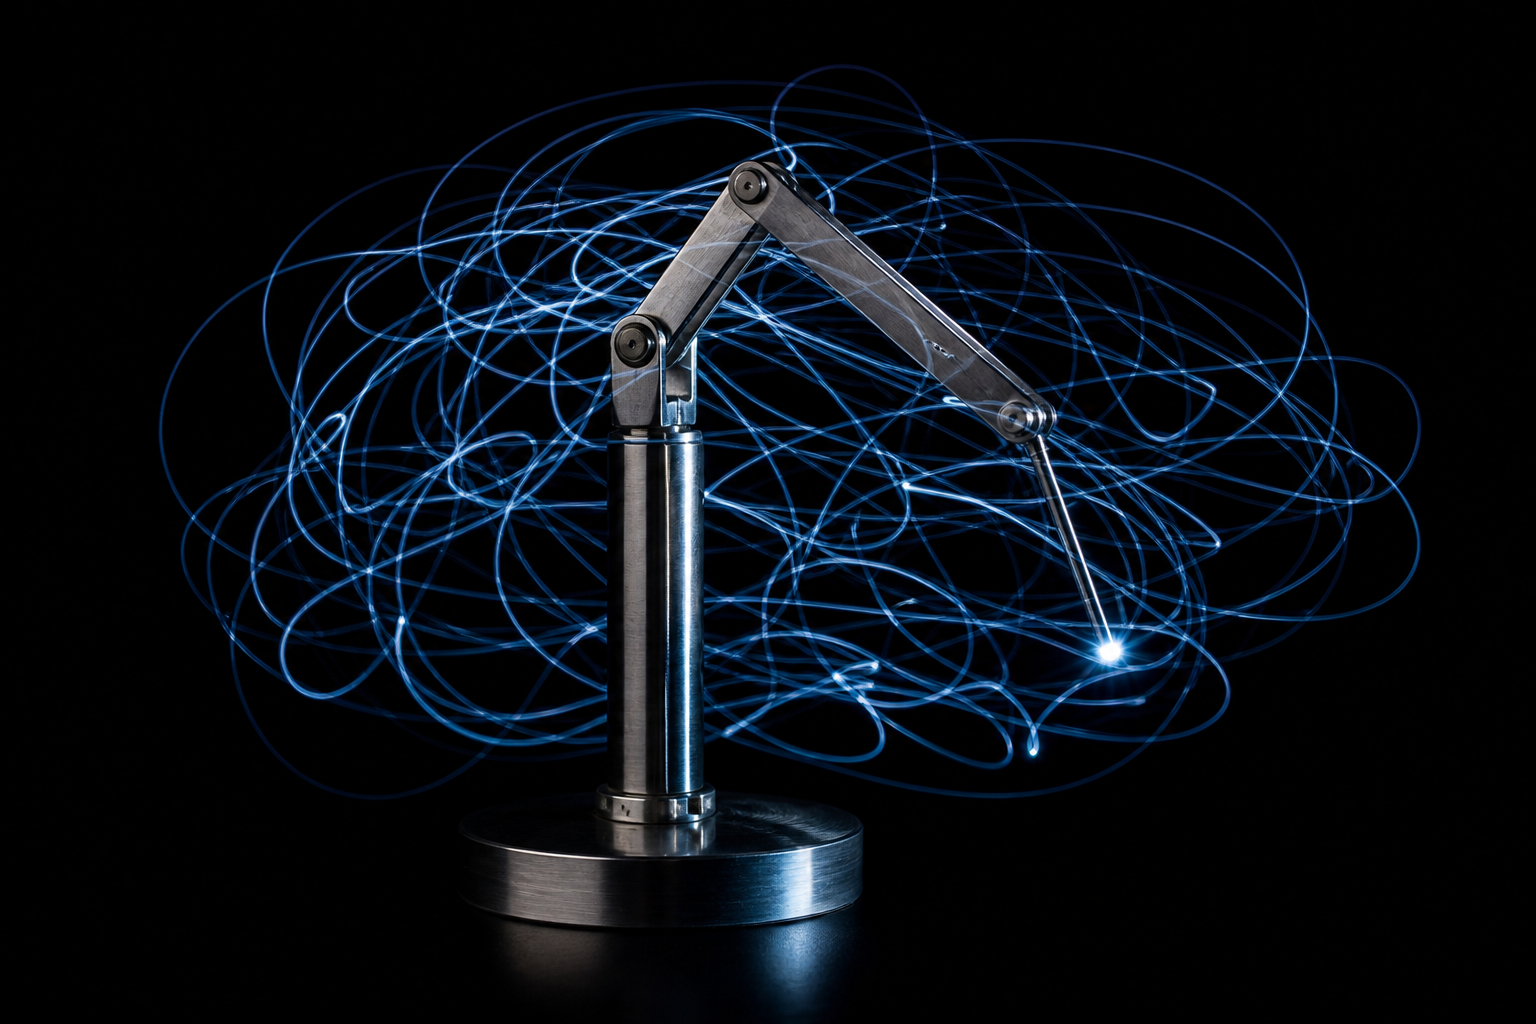
\includegraphics[width=0.58\linewidth]{images/book5/ai/b5-01-double-pendulum-trace.png}

{\small Um pêndulo duplo registrado por uma longa exposição: duas coordenadas, uma \omterm{def:b3:lagrangian-mechanics:action}{lagrangiana} e um movimento que nenhuma fórmula prevê por muito tempo --- a maquinaria da \omterm{thm:b3:lagrangian-mechanics:euler-lagrange}{mínima ação} deste capítulo escreve as equações; o caos mantém humildes as suas soluções.}
\end{omfigure}

\section{Exercícios}

\begin{exercise}[$\star$]\label{exo:b3:lagrangian-mechanics:1}
Conte os \omterm{def:b3:lagrangian-mechanics:coordinates}{graus de liberdade} e proponha \omterm{def:b3:lagrangian-mechanics:coordinates}{coordenadas generalizadas}: (a)
uma partícula no interior de uma tigela fixa; (b) um cilindro que rola
sem deslizar por um plano inclinado fixo; (c) um pêndulo duplo cujo
pivô superior desliza sobre um trilho horizontal; (d) um haltere (duas
massas, haste rígida) no espaço; (e) duas contas no mesmo arame
circular fixo. Qual \omterm{def:b3:lagrangian-mechanics:coordinates}{vínculo} desta lista relaciona velocidades em vez de
posições, e por que ele é, ainda assim, integrável a um \omterm{def:b3:lagrangian-mechanics:coordinates}{vínculo}
holônomo?
\end{exercise}

\begin{exercise}[$\star$]\label{exo:b3:lagrangian-mechanics:2}
Para o pêndulo plano (\cref{ex:b3:lagrangian-mechanics:pendulum}): (a)
verifique as dimensões de $L$ e de $p_\theta =
\partial L/\partial\dot\theta$; (b) identifique $p_\theta$ fisicamente;
(c) deduza o período para pequenos ângulos; (d) calcule a \omterm{def:b3:lagrangian-mechanics:action}{ação} $S$ de
uma oscilação pequena completa de amplitude $\theta_0$ --- e explique a
resposta antes de calcular (qual é a média temporal de $E_k - E_p$ numa
oscilação harmônica?).
\end{exercise}

\begin{exercise}[$\star$]\label{exo:b3:lagrangian-mechanics:3}
Uma máquina de Atwood: as massas $m_1$ e $m_2$ pendem de um fio ideal
que passa por uma polia sem massa. (a) Escolha uma coordenada e escreva
$L$. (b) Encontre a aceleração. (c) O tratamento de Newton precisava da
tração --- para onde ela foi? (d) Como você recuperaria a tração uma
vez conhecido o movimento?
\end{exercise}

\begin{exercise}[$\star$]\label{exo:b3:lagrangian-mechanics:4}
Uma partícula livre em coordenadas cilíndricas: $L = \tfrac12 m(\dot r^2 +
r^2\dot\varphi^2 + \dot z^2)$. (a) Quais coordenadas são cíclicas e
quais são os momentos conservados? (b) Por que $p_r$ \emph{não} se
conserva, embora nenhuma força atue? (c) Escreva a equação de
Euler--Lagrange para $r$ e interprete o termo $mr\dot\varphi^2$. (d)
Verifique que uma reta percorrida com velocidade constante a resolve.
\end{exercise}

\begin{exercise}[$\star\star$]\label{exo:b3:lagrangian-mechanics:5}
Um bloco de massa $m$ desliza sobre a face sem atrito (ângulo $\alpha$)
de uma cunha de massa $M$, ela própria livre para deslizar sobre um
piso sem atrito. (a) Escolha duas coordenadas: a abscissa $X$ da cunha
e a distância $s$ percorrida pelo bloco ao longo da face; escreva $L$.
(b) Qual coordenada é cíclica e que lei de conservação ela exprime?
(c) Encontre as duas acelerações. (d) Verifique os limites
$M \to \infty$ e $\alpha \to
90^\circ$.
\end{exercise}

\begin{exercise}[$\star\star$]\label{exo:b3:lagrangian-mechanics:6}
O pêndulo esférico: uma massa na ponta de uma haste de comprimento
$\ell$, livre nos dois ângulos ($\theta$ a partir da vertical
descendente, $\varphi$ em torno dela). (a) Escreva $L$. (b) Identifique
a \omterm{def:b3:lagrangian-mechanics:momentum}{coordenada cíclica} e o momento conservado $p_\varphi$. (c) Reduza o
movimento de $\theta$ a um potencial efetivo e esboce-o. (d) Para o
movimento cônico $\theta =
\theta_0$, recupere a relação do pêndulo cônico $\cos\theta_0 =
g/\ell\omega^2$ do volume do primeiro ano.
\end{exercise}

\begin{exercise}[$\star\star$]\label{exo:b3:lagrangian-mechanics:7}
Um pêndulo (massa $m$, comprimento $\ell$) pende de um carrinho de
massa $M$ livre para rolar sobre um trilho horizontal. (a) Com as
coordenadas $X$ (carrinho) e $\theta$, escreva $L$. (b) O que se
conserva, e por quê fisicamente? (c) Linearize para $\theta$ pequeno e
mostre que a frequência de oscilação é
$\Omega = \sqrt{(1 + m/M)\,g/\ell}$. (d) Explique os limites $M \to
\infty$ e $M \to 0$ --- por que um carrinho leve \emph{aumenta} a
frequência?
\end{exercise}

\begin{exercise}[$\star\star$]\label{exo:b3:lagrangian-mechanics:8}
Uma partícula de carga $q$ num campo uniforme $\vect B = B\vect e_z$,
descrito por $\vect A = \tfrac12\vect B\wedge\vect r$. (a) Escreva $L$
em coordenadas cartesianas. (b) Deduza as equações de movimento e
verifique que descrevem o círculo do cíclotron com
$\omega_{\text{c}} = qB/m$. (c) Calcule os momentos conjugados $p_x$ e
$p_y$: valem $m\dot x$ e $m\dot y$? Conservam-se? (d) Mostre que $L$
escrita em coordenadas cilíndricas tem $\varphi$ cíclica e identifique
o $p_\varphi$ conservado para um círculo centrado no eixo.
\end{exercise}

\begin{exercise}[$\star\star$]\label{exo:b3:lagrangian-mechanics:9}
Para a conta no aro que gira
(\cref{ex:b3:lagrangian-mechanics:hoop}): (a) calcule a \omterm{prop:b3:lagrangian-mechanics:energy}{função energia}
$h$ e verifique que a equação de movimento a conserva; (b) calcule a
energia mecânica $E$ e mostre que $E - h =
m\omega^2R^2\sin^2\theta$; (c) obtenha a potência fornecida pelo motor
em função de $\theta$ e $\dot\theta$; (d) obtenha a frequência das
\omterm{prop:b3:lagrangian-mechanics:modes}{pequenas oscilações} em torno do equilíbrio inclinado quando
$\omega^2 > g/R$ e mostre que ela se anula quando $\omega^2 \to g/R$
--- a lentidão que anuncia o desdobramento do poço.
\end{exercise}

\begin{exercise}[$\star\star\star$]\label{exo:b3:lagrangian-mechanics:10}
O pêndulo duplo igual ($m_1 = m_2 = m$, $\ell_1 = \ell_2 = \ell$). (a)
Mostre que, para pequenos ângulos, $L = \tfrac12 m\ell^2(2\dot\theta_1^2 +
2\dot\theta_1\dot\theta_2 + \dot\theta_2^2) - \tfrac12 mg\ell(2
\theta_1^2 + \theta_2^2)$. (b) Escreva as duas equações de movimento.
(c) Obtenha as frequências normais
$\Omega_\pm^2 = (2 \mp \sqrt2)\,g/\ell$ e a forma de cada modo
($\theta_2 = \pm\sqrt2\,\theta_1$). (d) Em grande amplitude, este
sistema é um exemplo clássico de caos: explique em poucas linhas o que
quebra a análise de pequenos ângulos e por que nenhuma lei de
conservação se perde.
\end{exercise}

\begin{exercise}[$\star\star\star$]\label{exo:b3:lagrangian-mechanics:11}
\emph{A braquistócrona.} Uma conta desliza sem atrito, partindo do
repouso na origem, por uma curva $y(x)$ ($y$ para baixo) até um ponto
$(a, b)$. (a) Usando a conservação da energia, mostre que o tempo de
descida é $T =
\int_0^a\sqrt{(1 + y'^2)/2gy}\,\dd x$ --- um funcional, com $x$ no
papel do tempo. (b) O integrando $F(y, y')$ não tem $x$ explícito:
mostre que $h = y'\,\partial F/\partial y' - F$ é constante ao longo da
curva ótima (o mesmo cálculo da
\cref{prop:b3:lagrangian-mechanics:energy}). (c) Deduza $y(1 + y'^2) =
2r$ para uma constante $r$ e verifique que a cicloide $x = r(\phi -
\sin\phi)$, $y = r(1 - \cos\phi)$ a satisfaz. (d) Mostre que a descida
da conta até o fundo de um arco leva $\pi\sqrt{r/g}$ e compare com a
rampa reta até o mesmo ponto.
\end{exercise}

\begin{exercise}[$\star\star\star$]\label{exo:b3:lagrangian-mechanics:12}
\emph{Fermat como \omterm{thm:b3:lagrangian-mechanics:euler-lagrange}{mínima ação}.} A luz num meio de índice $n(y)$ viaja
entre dois pontos no menor tempo (volume do segundo ano). (a) Mostre
que o tempo de percurso ao longo de $y(x)$ é $T = \tfrac1c\int n(y)\sqrt{1 +
y'^2}\,\dd x$. (b) Como o integrando não tem $x$ explícito, use o $h$
conservado do exercício anterior para mostrar que $n(y)\big/\sqrt{1 +
y'^2} = \text{const}$, e verifique que isso é a lei de Snell $n\sin i =
\text{const}$ para um raio medido a partir da vertical. (c) Sobre uma
estrada quente, o índice cresce com a altura como
$n(y) \approx n_0(1 + \beta y)$; mostre que um raio quase horizontal se
encurva com raio de curvatura $R \approx
1/\beta$. (d) Com $\beta = \qty{1.2e-5}{m^{-1}}$, de que distância um
motorista cujos olhos estão a \qty{1.2}{m} acima da estrada vê nela a
miragem de ``água''?
\end{exercise}

\begin{omfigure}
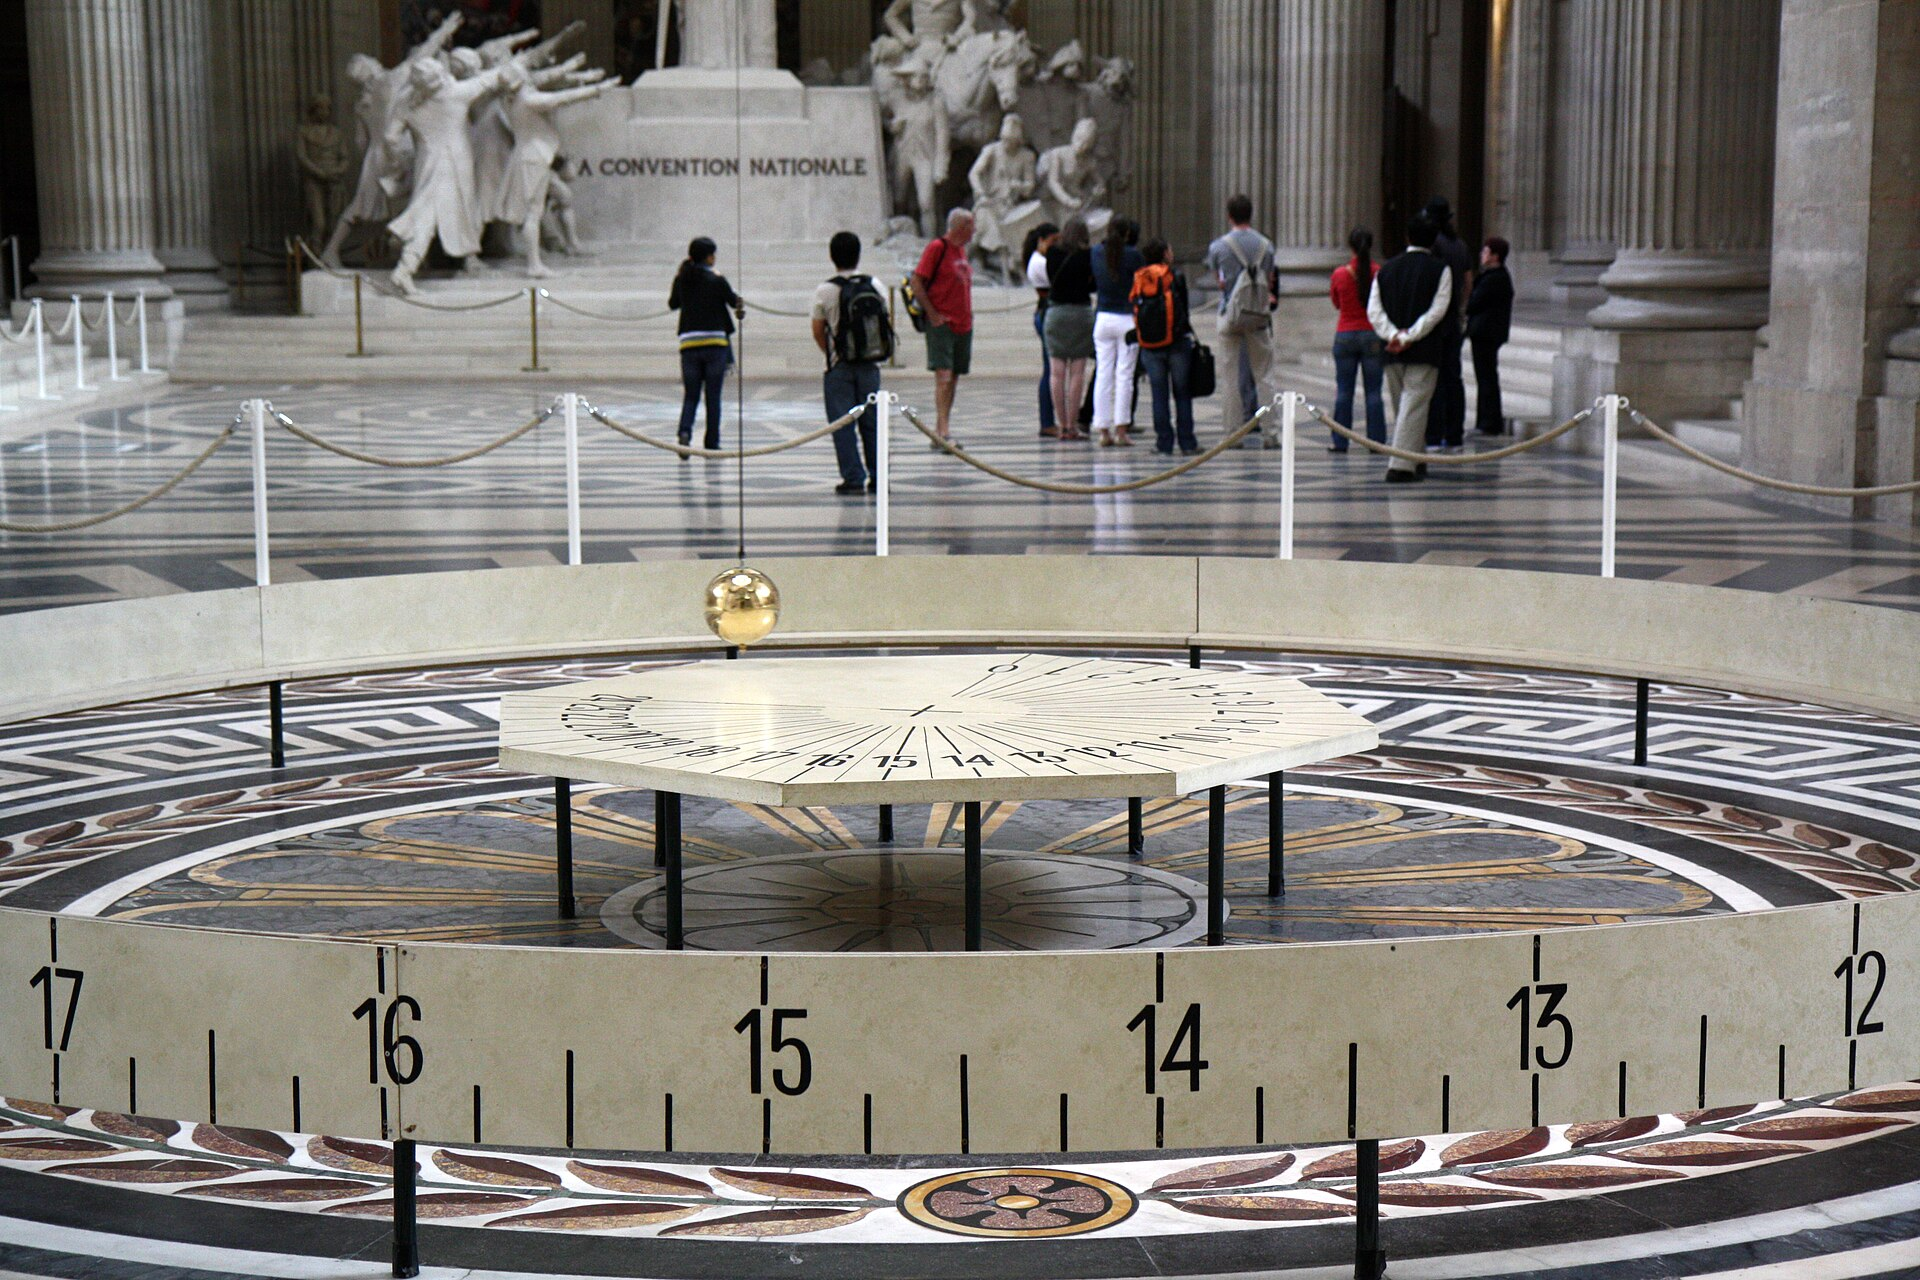
\includegraphics[width=0.6\linewidth]{images/book5/photo-foucault-pantheon.jpg}

{\small O pêndulo de Foucault no Panteão, em Paris. \omterm{def:b3:lagrangian-mechanics:coordinates}{Coordenadas generalizadas}, um \omterm{def:b3:lagrangian-mechanics:coordinates}{vínculo} e um referencial que gira lentamente: a rotação da sala aparece nas equações de movimento --- e a deriva do plano de oscilação permite que um porão meça a rotação da Terra. Fotografia: Olga Khomitsevich, CC~BY~2.0.}
\end{omfigure}

\section{Problema: A vassoura que fica de cabeça para baixo}

\begin{problem}[{Problema de fim de semana --- O pêndulo invertido de Kapitza}]\label{pb:b3:lagrangian-mechanics:1}
Um pêndulo rígido pode permanecer estável \emph{acima} de seu pivô se
este for sacudido para cima e para baixo com rapidez suficiente ---
descoberta analisada por Kapitza em 1951, surpreendente a ponto de
parecer um truque de mágica, e o princípio pelo qual campos elétricos
oscilantes aprisionam íons isolados. Modelamos o pêndulo como uma massa
pontual $m$ na extremidade de uma haste rígida sem massa de comprimento
$\ell = \qty{40}{cm}$; $\theta$ é o ângulo a partir da vertical
\emph{descendente}; $g = \qty{9.81}{m/s^2}$.

\medskip\noindent\textbf{Parte I --- O pêndulo rígido.}
De início, o pivô é mantido fixo.
\begin{enumerate}
  \item Escreva a \omterm{def:b3:lagrangian-mechanics:action}{lagrangiana} e a equação de movimento.
  \item Dê a frequência $f_0$ das \omterm{prop:b3:lagrangian-mechanics:modes}{pequenas oscilações} em torno de $\theta =
        0$, e seu valor.
  \item Mostre que aqui $h = E$ e use sua conservação para achar a
        velocidade mínima de lançamento da massa, no ponto mais baixo,
        que a leva até o topo.
  \item Linearize a equação perto de $\theta = \pi$ (ponha $\theta = \pi +
        \epsilon$) e mostre que $\ddot\epsilon = +(g/\ell)\epsilon$:
        com que rapidez cresce uma inclinação inicial de um milésimo
        de grau? Dê o tempo para que ela cresça por um fator $e$.
  \item Uma vassoura equilibrada na ponta do dedo cai em cerca de um
        segundo e nunca se sustenta sozinha: diga numa frase o que a
        equação linearizada afirma sobre o equilíbrio $\theta = \pi$.
\end{enumerate}

\medskip\noindent\textbf{Parte II --- Sacudindo o pivô.}
O pivô agora oscila verticalmente, com altura $y_{\text{s}}(t) =
a\cos\Omega t$, sendo $a = \qty{2.0}{cm}$ e $\Omega$ ajustável.
\begin{enumerate}[resume]
  \item Escreva as coordenadas da massa e mostre que
        $\vect v^{\,2} = \ell^2\dot\theta^2 -
        2a\Omega\ell\sin(\Omega t)\sin\theta\,\dot\theta +
        a^2\Omega^2\sin^2\Omega t$.
  \item Mostre que duas \omterm{def:b3:lagrangian-mechanics:action}{lagrangianas} que diferem por uma derivada
        temporal total $\dd F(q,t)/\dd t$ dão as mesmas \omterm{thm:b3:lagrangian-mechanics:euler-lagrange}{equações de
        Euler--Lagrange}.
  \item Usando essa liberdade, reduza a \omterm{def:b3:lagrangian-mechanics:action}{lagrangiana} a $L = \tfrac12 m
        \ell^2\dot\theta^2 - ma\Omega^2\ell\cos(\Omega t)\cos\theta +
        mg\ell\cos\theta$. (Sugestão: $\sin(\Omega t)\sin\theta\,\dot\theta$
        combina-se com um termo $\cos(\Omega t)\cos\theta$ numa derivada
        total; termos que dependem só de $t$ podem ser descartados.)
  \item Deduza a equação de movimento
        \[
        \ddot\theta = -\frac{g}{\ell}\sin\theta
         + \frac{a\Omega^2}{\ell}\cos(\Omega t)\sin\theta .
        \]
        Interprete o segundo termo como a substituição do peso por $g +
        \ddot y_{\text{s}}$: o pêndulo vive num elevador.
  \item A \omterm{prop:b3:lagrangian-mechanics:energy}{função energia} $h$ ainda se conserva? E a energia? O que
        bombeia energia para dentro e para fora?
  \item No regime de Kapitza, $a \ll \ell$ e $\Omega \gg \omega_0 =
        \sqrt{g/\ell}$: verifique-os para $a = \qty{2}{cm}$, $\ell =
        \qty{40}{cm}$, $\Omega/2\pi = \qty{40}{Hz}$, e explique
        fisicamente por que a massa não consegue acompanhar a excitação.
\end{enumerate}

\medskip\noindent\textbf{Parte III --- Separando o rápido do lento.}
Procure o movimento na forma $\theta(t) = \Theta(t) + \xi(t)$: uma
deriva lenta $\Theta$ mais uma pequena ondulação $\xi$ na frequência de
excitação.
\begin{enumerate}[resume]
  \item Mantendo apenas o maior termo de cada lado, mostre que a
        ondulação obedece a $\ddot\xi \approx +(a\Omega^2/\ell)\cos(\Omega t)
        \sin\Theta$, com $\Theta$ congelado na escala de tempo da
        excitação.
  \item Deduza $\xi(t) = -(a/\ell)\cos(\Omega t)\sin\Theta$ e verifique
        que sua amplitude é pequena, da ordem de $a/\ell$.
  \item Expanda $\sin\theta = \sin(\Theta + \xi)$ em primeira ordem em
        $\xi$ e insira o resultado na equação de movimento.
  \item Faça a média sobre um período de excitação, com $\Theta$ fixo:
        usando $\langle\cos\Omega t\rangle = 0$ e
        $\langle\cos^2\Omega t\rangle = \tfrac12$, mostre que
        \[
        \ddot\Theta = -\frac{g}{\ell}\sin\Theta
         - \frac{a^2\Omega^2}{2\ell^2}\sin\Theta\cos\Theta .
        \]
  \item Mostre que isso é um movimento na \omterm{ex:b3:lagrangian-mechanics:hoop}{energia potencial efetiva}
        \[
        U_{\text{eff}}(\Theta) = mg\ell\Big({-\cos\Theta}
         + \frac{a^2\Omega^2}{4g\ell}\sin^2\Theta\Big) .
        \]
  \item Compare com a conta no aro que gira
        (\cref{ex:b3:lagrangian-mechanics:hoop}): a mesma matemática,
        com sinal oposto no termo novo --- o que a sacudida faz ao
        equilíbrio \emph{de baixo} que a rotação não fazia?
  \item Esboce $U_{\text{eff}}$ para excitação lenta e para excitação
        rápida e descreva cada equilíbrio e sua estabilidade em cada caso.
\end{enumerate}

\medskip\noindent\textbf{Parte IV --- A vassoura se levanta.}
\begin{enumerate}[resume]
  \item Expandindo $U_{\text{eff}}$ perto de $\Theta = \pi$, mostre que
        a posição invertida é estável exatamente quando
        \[
        a^2\Omega^2 > 2g\ell .
        \]
  \item Calcule a frequência crítica de excitação $f_{\text{c}} =
        \Omega_{\text{c}}/2\pi$ para o nosso pêndulo, bem como a
        velocidade máxima do pivô $a\Omega_{\text{c}}$ e a aceleração
        $a\Omega_{\text{c}}^2$ (em unidades de $g$) que ela exige.
  \item Em $\Omega = 2\Omega_{\text{c}}$, obtenha a frequência da
        oscilação lenta do pêndulo em pé em torno de $\Theta = \pi$ e
        seu valor; verifique que ela é de fato lenta em comparação
        com a excitação.
  \item Ainda em $\Omega = 2\Omega_{\text{c}}$, qual é a amplitude da
        ondulação $\xi$ com $\Theta$ pouco afastado de $\pi$, em graus,
        para $a/\ell = 0.05$? Uma fotografia denunciaria o truque?
  \item Quanto a vassoura pode inclinar-se em relação à vertical e
        ainda voltar? Mostre que o poço da posição em pé se estende
        por $|\Theta - \pi| <
        \arccos(2g\ell/a^2\Omega^2)$, e avalie-o em $\Omega =
        2\Omega_{\text{c}}$.
  \item Um malabarista que equilibra uma vassoura na ponta de um dedo
        imóvel também a mantém em pé --- por qual mecanismo
        inteiramente diferente? Nomeie a característica do pêndulo de
        Kapitza que dispensa realimentação.
  \item Resuma o resultado central: um pivô sacudido com amplitude
        \qty{2}{cm} a \qty{45}{Hz} --- o dobro da frequência crítica
        --- mantém de cabeça para baixo um pêndulo de \qty{40}{cm},
        num poço que alcança cerca de $75^\circ$ a partir da vertical,
        balançando suavemente a cerca de \qty{1.4}{Hz}. Onde na física
        se usa esse mesmo aprisionamento em média para segurar uma
        única partícula carregada?
\end{enumerate}
\end{problem}
